\section{Introduction}

\begin{figure*}

  \begin{panel}{(a)}{\textwidth}
    \vspace{5mm}
    \small
    \tikzsetnextfilename{figure_1_overview}
    \usetikzlibrary{spy}%
\def\blinky#1#2#3#4#5{%
  \begin{tikzpicture}[node distance=3mm]
    \node[site#1] (s1) {};
    \node[site#2,right of=s1] (s2) {};
    \coordinate (s12) at ($(s1)!.5!(s2)$);
    \node[site#3,right of=s2] (s3) {};
    \node[site#4,below of=s12] (s4) {};
    \node[site#5,right of=s4] (s5) {};
    \foreach \angle in {0, 45, 90, 135, 180, 225, 270, 315}{
      \begin{scope}[rotate=\angle]
        \draw[sitelight#1] ($(s1)+(0,0.13)$) -- ($(s1)+(0,0.16)$);
        \draw[sitelight#2] ($(s2)+(0,0.13)$) -- ($(s2)+(0,0.16)$);
        \draw[sitelight#3] ($(s3)+(0,0.13)$) -- ($(s3)+(0,0.16)$);
        \draw[sitelight#4] ($(s4)+(0,0.13)$) -- ($(s4)+(0,0.16)$);
        \draw[sitelight#5] ($(s5)+(0,0.13)$) -- ($(s5)+(0,0.16)$);
      \end{scope}
    }
  \end{tikzpicture}
}%
\begin{tikzpicture}

  \begin{scope}[spy using outlines={magnification=2,size=12mm,very thick}]

    \node[image] (frame) {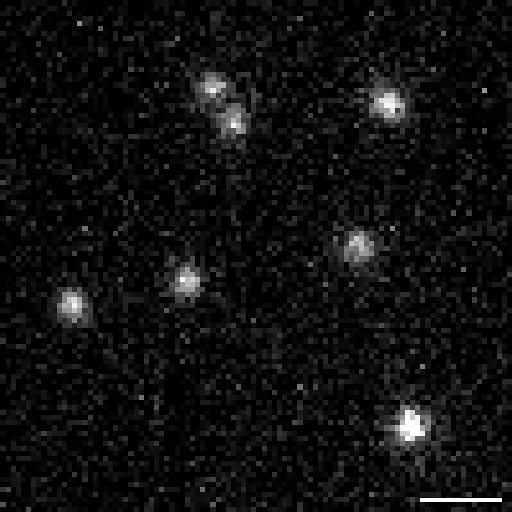
\includegraphics[width=4cm]{figures/data/overview/sample_frame}};

    \spy on ($(frame)+(1.1, 1.2)$)
      in node (patch_3) [image,right=6mm,anchor=north west]
      at (frame.north east);
    \spy on ($(frame)+(0.9, 1.1)$)
      in node (patch_2) [image,right=6mm,anchor=north west]
      at ($(frame.north east)-(0.1,0.1)$);
    \spy[
        draw=funkey_color_1,
        every spy on node/.append style={ultra thick},
        every spy in node/.append style={ultra thick},
        spy connection path={\draw[ultra thick] (tikzspyonnode) -- (tikzspyinnode);}
    ]
      on ($(frame)+(1.0, 1.2)$)
      in node (patch_1) [image,right=6mm,anchor=north west]
      at ($(frame.north east)-(0.2,0.2)$);
  \end{scope}

  % example trace
  \node[right=4mm,anchor=north west,text width=6cm,inner sep=0] (trace) at (patch_3.north east) {%
    \def\tracecsv{figures/data/overview/trace.csv}%
    \def\traceintensitycol{trace}%
    \def\nolabels{}%
    \tikzexternaldisable%
    \centerline{\begin{tikzpicture}%
  \begin{axis}[
    name=trace,
    width=0.8\textwidth,
    height=5cm,
    xlabel=frames,
    ylabel=intensity,
    enlarge x limits=false,
    xtick distance=500,
    grid=major,
    grid style={dashed},
    scaled ticks=false,
    ticklabel style={font=\small},
    legend style={nodes={scale=0.6, transform shape}},
  ]

    \addplot [
      color=tracecolor,
      mark=*,
      mark size=0.7pt,
      mark options={line width=0},
      fill opacity=0.8,
      draw opacity=0.2,
    ] table [
      col sep=comma,
      x=frames,
      y=\traceintensitycol
    ] {\tracecsv};
    \addlegendentry{intensity trace}

    \addplot [
      color=ztracecolor,
      thick
    ] table [
      col sep=comma,
      x=frames,
      y=\zcol
    ] {\tracecsv};
    \addlegendentry{inferred state}

    % remember min/max y-axis values for next plot
    \pgfplotsextra{
      \pgfmathparse{\pgfkeysvalueof{/pgfplots/ymin}}
      \global\let\ymin\pgfmathresult
      \pgfmathparse{\pgfkeysvalueof{/pgfplots/ymax}}
      \global\let\ymax\pgfmathresult
    }

  \end{axis}

  \begin{axis}[
    at={($(trace.east) + (4mm,0)$)},
    anchor=west,
    width=0.3\textwidth,
    height=5cm,
    yticklabel=\empty,
    xtick distance=0.005,
    xlabel=probability,
    grid=major,
    grid style={dashed, very thin},
    enlarge x limits={value=0.1,upper},
    scaled ticks=false,
    ymin=\ymin,
    ymax=\ymax,
    ticklabel style={font=\small},
    legend style={nodes={scale=0.6, transform shape}},
  ]

    \addplot+[
      xbar interval,
      mark=none,
      color=tracecolor,
      fill=tracecolor,
      fill opacity=0.6,
      draw=none,
    ] table [
      col sep=comma,
      y=\histbincol,
      x=\histcountcol,
    ] {\histogramcsv};
    \addlegendentry{intensity histogram}

    \addplot[
      color=intensitymodelcolor!80!black,
      thick
    ] table [
      col sep=comma,
      y=\histbincol,
      x=\modelfitcol
    ] {\histogramcsv};
    \addlegendentry{inferred model}

  \end{axis}
\end{tikzpicture}%
}%
    \tikzexternalenable%
  };
  \node[anchor=north,inner sep=0pt] at (trace.230) {\tiny time};
  \node[rotate=90,anchor=south,inner sep=1pt] at (trace.west) {\tiny intensity};

  % observed / hidden line
  \draw[gray,very thick]
    (patch_1.west|-frame.355) --
      node[pos=0,anchor=south west] {observed}
      node[pos=0,anchor=north west] {hidden}
      node[pos=0.35] (sample_1) {}
      node[pos=0.60] (sample_2) {}
      node[pos=0.96] (sample_3) {}
    (trace.east|-frame.355);

  % brace to MLE
  \draw[decorate,decoration={brace,raise=2mm}]
    (trace.north east) --
    node[pos=0.5,right=5mm,draw,rectangle,rounded corners] (mle) {\ours}
    (trace.south east);

  % posterior
  \node[anchor=north west,text width=3.6cm] (posterior) at ($(trace.north east)+(1.8,0.3)$) {%
    \def\posteriorcsv{figures/data/overview/posterior.csv}%
    \def\posteriorcol{posterior}%
    \def\noylabels{}%
    \tikzexternaldisable%
    \@ifundefined{noylabels}{}{%
  \pgfplotsset{yticklabel=\empty}%
}%
\begin{tikzpicture}%

  \def\eps{0.001}

  \begin{axis}[
    width=\textwidth,
    height=\textwidth,
    xlabel=\n,
    xlabel=$p(\n|\trace)$,
    grid=major,
    grid style={dashed, very thin},
    enlarge x limits=0.1,
    enlarge y limits=0,
    ymin=0,
    ymax=1,
    scaled ticks=false,
    ticklabel style={font=\small},
  ]

    \addplot+[
      ybar,
      bar width=1,
      mark=none,
      fill=posteriorcolor,
      fill opacity=0.6,
      draw=posteriorcolor,
      y filter/.expression={
        y < \eps ? nan : y
      },
    ] table [
      col sep=comma,
      y=\posteriorcol,
      x=n,
    ] {\posteriorcsv};

    \ifdefined\posteriorcolextra
      \addplot+[
        ybar,
        bar width=1,
        mark=none,
        fill=posteriorcolor!60!black,
        fill opacity=0.6,
        draw=posteriorcolor,
        y filter/.expression={
          y < \eps ? nan : y
        },
      ] table [
        col sep=comma,
        y=\posteriorcolextra,
        x=n,
      ] {\posteriorcsv};
    \fi

  \end{axis}

\end{tikzpicture}
%
    \tikzexternalenable%
  };
  \draw[arrow,shorten >=-8] (mle) -- (mle-|posterior.west);

  % blinky things
  \node (hidden) at (frame.330-|patch_1) {\blinky{off}{off}{off}{off}{off}};
  \node (z_sample_1) at (frame.330-|sample_1) {\blinky{on}{off}{on}{on}{off}};
  \node (z_sample_2) at (frame.330-|sample_2) {\blinky{on}{off}{on}{off}{off}};
  \node (z_sample_3) at (frame.330-|sample_3) {\blinky{on}{off}{off}{off}{off}};

  \draw[arrow] (z_sample_1) -- +(0, 2.4);
  \draw[arrow] (z_sample_2) -- +(0, 2.05);
  \draw[arrow] (z_sample_3) -- +(0, 1.7);

  \node[anchor=north,inner sep=10pt] at (hidden) {\strut$\n=5$};
  \node[anchor=north,inner sep=10pt] at (z_sample_1) {\strut$\z{}=3$};
  \node[anchor=north,inner sep=10pt] at (z_sample_2) {\strut$\z{}=2$};
  \node[anchor=north,inner sep=10pt] at (z_sample_3) {\strut$\z{}=1$};

\end{tikzpicture}

    \vspace{-2mm}
  \end{panel}

  \begin{panel}{(b)}{0.6\textwidth}
    \begin{panel}{}{\textwidth}
      \small
      \tikzsetnextfilename{figure_1_p_on_off}
      \centerline{\begin{tikzpicture}
  \node[siteoff,inner sep=4pt] (off) {};
  \node[siteon,right=2cm of off,inner sep=4pt] (on) {};
  \foreach \angle in {0, 45, 90, 135, 180, 225, 270, 315}{
    \begin{scope}[rotate=\angle]
      \draw[sitelighton,ultra thick] ($(on)+(0,0.26)$) -- ($(on)+(0,0.32)$);
    \end{scope}
  }
  \draw[arrow,shorten >=2mm,shorten <=2mm] (off) to[bend left] node[pos=0.5,above] (pon) {\pon} (on);
  \draw[arrow,shorten >=2mm,shorten <=2mm] (on) to[bend left] node[pos=0.5,below] {\poff} (off);

  \node[right=14mm of on] (re) {$\sim\poisson(\re\deltat)$};
  \draw[arrow,decorate,decoration={coil,aspect=0,segment length=6,post=curveto,post length=2mm}] ($(on.east)+(0.2,0)$) -- (re);

  %\node[parameters,anchor=south] at (re.north) {\strut$\parameterst = (\pon, \poff)$};

  \node[above=1mm of pon,gray] {transition model};
\end{tikzpicture}
}
    \end{panel}

    \vspace{4mm}
    \begin{panel}{(c)}{\textwidth}
      \small
      \hspace{4mm}
      \tikzsetnextfilename{figure_1_intensity_model}
      \begin{tikzpicture}

  \node (z) {\blinky{on}{off}{on}{on}{off}};
  \node[var,right=18mm of z] (c) {$\photons$};
  \node[annotation,below of=c] (c_dist) {$\sim\poisson((\z{}\re + \rb)\deltat)$};
  \draw (c) -- (c_dist);
  \draw[arrow,decorate,decoration={coil,aspect=0,segment length=6,post=curveto,post length=3mm}]
    (z.east) -- (c);

  \node[right=12mm of c,inner sep=0,yshift=2mm] (camera) {
    \tikz[plane x={(0.8,-0.4)},canvas is plane,transform shape]{
      \draw[gray,step=0.25] (0, 0) grid (1, 1);
      \node[anchor=south,gray] at (0.5, 1.1) {detector};
    }
  };

  \coordinate (camera_center) at (camera.center|-c);
  \draw[arrow,shorten >=3mm] (c) -- (camera_center);
  \node[observation,right=18mm of camera_center] (x) {$\x{}$};
  \node[annotation,below of=x] (x_dist) {$\sim\mathcal{N}(\photons\camgain + \camoffset, \camvar)$};
  \draw (x) -- (x_dist);
  \draw[arrow] (camera.east|-c) -- (x);
  \node[below=1mm of z] {\z{}};

  % parameter collections
  %\node[parameters,anchor=south west] at (z.north east) {\strut$\parameterse = (\re, \rb)$};
  %\node[parameters,anchor=south east] at (z.north-|x_dist.east) {\strut$\parametersc = (\camgain, \camoffset, \camvar)$};

  % annotations
  \node[above=2mm of c,gray] {\strut emission model};
  \node[above=2mm of x,gray] {\strut camera model};
\end{tikzpicture}

    \end{panel}
  \end{panel}
  \begin{panel}{(d)}{0.35\textwidth}
    \small
    \vspace{4mm}
    \hspace{4mm}
    \tikzsetnextfilename{figure_1_model}
    \centerline{\begin{tikzpicture}

  % parameters
  \node[var] (n) {\n};
  \node[var,below of=n] (theta_T) {\parameterst};
  \node[var,below of=theta_T] (theta_E) {\parameterse};
  \node[var,below of=theta_E] (theta_C) {\parametersc};

  % hidden states
  \node[state,right=1cm] (z1) at ($(n)!.5!(theta_T)$) {\z{1}};
  \node[state,right=4mm of z1] (z2) {\z{2}};
  \node[state,right=1cm of z2] (zt) {\z{t}};
  \node at ($(z2)!.5!(zt)$) {$\cdots$};

  % observations
  \node[observation,right=1cm] (x1) at ($(theta_E)!.5!(theta_C)$) {\x{1}};
  \node[observation,right=4mm of x1] (x2) {\x{2}};
  \node[observation,right=1cm of x2] (xt) {\x{t}};
  \node at ($(x2)!.5!(xt)$) {$\cdots$};

  % plates
  \begin{pgfonlayer}{background}
    \node[plate,fit=(z1)(zt)] (hidden) {};
    \node[plate,fit=(x1)(xt)] (observed) {};
  \end{pgfonlayer}

  % dependencies
  \draw[arrow] (n) to (hidden);
  \draw[arrow] (theta_T) to (hidden);
  \draw[arrow] (theta_E) to (observed);
  \draw[arrow] (theta_C) to (observed);
  \draw[arrow] (z1) to (x1);
  \draw[arrow] (z2) to (x2);
  \draw[arrow] (zt) to (xt);
  \draw[arrow] (z1) to (z2);
  \draw[arrow,shorten <=20] (z2) to (zt);
  \draw[shorten >=22] (z2) to (zt);

  % annotation
  \node[below of=observed] {$p(\trace|\n,\parameterst,\parameterse,\parametersc)$};

\end{tikzpicture}
}
  \end{panel}

  \caption{
      \panelref{a} Overview of the blinx method (scale bar: 1 $\mu$m)
      %
      \panelref{b} TODO
      %
      \panelref{c} TODO
      %
      \panelref{d} TODO \ours is based on a Hidden Markov Model who's
      parameters are optimized to build the final posterior distribution
  }
  \label{fig:method:overview}
\end{figure*}


% molecular counting: what is it and why do we care?
%
Molecular counting aims to determine the absolute number of \smallobjects
associated in an complex, a quantity that is often essential to understanding
the underlying biology of a system.
  %
  The activation of T cells, for example, is sensitive to single ligands, and
  quantifying the molecular count of ligand-receptor interactions informs
  understanding of system sensitivity and activation of downstream signalling 
  pathways~\citep{irvine_2002}.
  %
  Furthermore, molecular counting enables identification of oligomeric states by
  counting the subunits in a cluster, allowing differentiation of monomers, dimers,
  trimers, and higher order oligomers.
  %
  Several biological processes depend on oligomer quantity: TGF-$\beta$ signaling,
  for example, depends on the oligomeric state of Smad~\citep{inman_2002,
  moustakas_2002}.
  %
  Similarly, the oligomeric state of G-protein coupled receptors influences
  downstream GPCR signaling~\citep{felce_2018, breitwieser_2004}.

% fluorescence microscopy alone is not enough
%
Often, as in the aforementioned examples, the \smallobjects of interest are separated by only a few
nanometers and thus can not be quantified through standard fluorescence
microscopy techniques.
  %
  %Fluorescence microscopy can provide precise localization information of
  %molecular species, but its ability to determine quantitative information, such
  %as counts of nearby molecules, remains limited.
  %
  In contrast to larger structures (whole cells or organelles), which can
  be discerned in fluorescence microscopy, individual molecules in
  diffraction limited spots below a resolution of approximately 200 \nanometer can not
  be separated with light microscopy.
  %
  \todo{make positive statement}
  Even super-resolution techniques~\citep{betzig_2006,rust_2006,rittweger_sted_2009} cannot discern 
  \smallobjects that are closer than 10 \nanometer apart~\citep{valli_seeing_2021}.
  \todo{this works up to a given distance}
  \todo{below that distance, SR methods can not count molecules any longer}

\todo{make clear: we are interested in counts, not structure; SR is for structure, not counts}

% summary of what the problem is and how we approach it
%
We present an alternative to counting the number of molecules in a diffraction
limited spot, which does not rely on super-resolution.
%
  To that end, we develop a Bayesian solution to estimate the number of
  fluorescently labelled \smallobjects directly from a diffraction limited
  spot.
  %
  Our solution is based on a probabilistic model that incorporates the
  photo-physics of blinking fluorescent emitters and models their dynamics over
  time as a Markov chain.
  %
  Given a trace of the combined intensity of all \smallobjects contained in a
  spot over time (\figref{fig:method:overview}a), this model can be used to obtain the 
  most likely number of emitters contained in that spot: the molecular count.

% Motivate fluorescence based methods (doesn't say a lot IMO -Jan)
%
%
%Although other methods exist to quantify molecular count at this scale, a
%robust, accurate, \todo{needs citations} fluorescence based method would make
%quantification much more accessible, while maintaining the benefits of
%fluorescence imaging, such as spatial localization.

%%%%%%%%%%%%%%%%
% Related Work %
%%%%%%%%%%%%%%%%

% fluorescence intensity based counting
%
Perhaps the simplest method of molecular counting is to correlate the combined
fluorescent intensity of a spot with the number of \smallobjects, \ie, the more subunits 
located within a spot, the brighter the spot is expected to be ~\citep{schmied_2012,
tolar_2005}.
  %
  This method works well for qualitative measurements, but, due to the noise in
  intensities measured from any single fluorophore, this approach lacks the precision 
  required for accurate estimates of molecular counts. 

% Other methods work by separating things out in time
%
Molecular counting methods that incorporate temporal fluctuations of intensity
are more accurate than correlation approaches.
  %
  % FCS and bSOFI
  Methods such as fluorescence correlation spectroscopy
  (FCS)~\citep{otsuka_2023,wachsmuth_2015,politi_2018} and balanced
  super-resolution optical fluctuation imaging
  (bSOFI)~\citep{geissbuehler_2012} fit higher order statistics to fluctuations
  in fluorescent intensity over time to quantify the molecular concentration.
  % Bleaching based
  In other methods, temporal variations in intensity are induced rather than
  just observed; for example, counting distinct bleaching
  steps can provide estimates of the number of fluorescent
  emitters~\citep{ulbrich_2007,jain_2011,hummert_2021, garry_bayesian_2020}.

% Some of those use blinking fluorophores
%
Blinking fluorophores, such as those used in
PALM~\citep{sengupta_pcPALM_2011,lee_counting_2012} and
STORM~\citep{patel_blinking_2021}, can be used to facilitate solving the counting
problem~\citep{rollins_stochastic_2015,nino_2017}.
  %
  % Some of these methods are also based on HMMs, should we mention that here?
  The blinking behavior allows for modeling at the single-molecule level, compared 
  to the bulk measurements of FCS, while the repeated transitions in
  intensity provide more information than the irreversible switches that occur 
  in bleaching-based counting.
  %
  % Limitations
  A major limitation of these methods is the complex photophysical properties of 
  these blinking fluorophores, making it difficult to differentiate between possible 
  dark states, and photo-bleaching. 

% DNA-PAINT is extra useful because its emitters don't bleach either
%
In contrast, DNA-PAINT~\citep{schnitzbauer_2017} achieves blinking through transient 
DNA-binding, effectively decoupling blinking from photophysics. Additionally this has 
the advantage of producing blinking fluorescence that is functionally immune to 
photo-bleaching due to the continuous replenishment of fluorophores from 
solution~\citep{stehr_2021}.

% In contrast, DNA-PAINT~\citep{schnitzbauer_2017} provides
% blinking fluorescence that is functionally immune to photo-bleaching due to the
% continuous replenishment of fluorophores from solution~\citep{stehr_2021}.
  % qPAINT
  Quantitative DNA-PAINT (qPAINT)~\citep{jungmann_2016} estimates the molecular
  count based on the frequency of blinking events. For example, if a blinking rate of one
  event per second is calibrated to one molecule, an observation of
  ten events per second corresponds to a count of ten molecules. 
  qPAINT is a relative counting method, and as a result is entirely dependant on the quality of 
  the calibration, which the measurement of is non-trivial.
  %
  % lbFCS
  Localization based FCS (\lbfcs)~\citep{stein_2019,stein_2021} combines the
  structured blinking of DNA-PAINT with the principles of FCS, fitting the
  autocorrelation function of intensity over time to produce a count. As such,
  it is able to accurately count up to six molecules in a single diffraction
  limited spot, without the need for a calibration.
  %
  % Limitations
  However, both of these methods are limited in that they fit summary
  statistics, rather than the data directly.
  %
  In contrast, our solution fits the model to each frame of the measurement 
  in sequence, fully utilizing both the temporal and intensity information available.
  
Furthermore, all prior methods provide a single estimate of molecular count, whereas 
a probabilistic method would provide valuable information for downstream analysis.
  %
  Bayesian approaches can estimate a likelihood for each possible condition 
  and have previously been used to infer the number of FRET conformational 
  states \citep{hon_bayesian-estimated_2019, bronson_learning_2009}, 
  the number of photo-bleaching steps \citep{garry_bayesian_2020},
  the assignment of blinking events to specific fluorophores \citep{gabitto_bayesian_2021, fazel_bayesian_2019},
  and the molecular count from observed intensity \citep{nino_2017}.

% Our Model
% ----------
% fully Bayesian
We propose \ours, a Bayesian model to estimate the molecular count
directly from a fluctuating sequence of fluorescent intensity measurements over
time.
  %
  % Based on a fully differentiable markov chain
  Based on a fully differentiable \hmm, \ours fits
  seven parameters that describe the photo-physics and kinetics of the system, 
  directly to the sequence of measurements and
  estimates a likelihood for each possible count.
  %
  % probabilistic
  These likelihoods can be compared directly, producing a posterior
  distribution of counts given the observation sequence.
  % more accurate than existing methods 
  We first run \ours as a forward model, to simulate
  different experimental conditions and determine their effects on counting ability.
  %
  We demonstrate a substantial improvement in calibration free (compared to \lbfcs) 
  and calibrated (compared to \qpaint), counting accuracy, and 
  an ability to count across different kinetic regimes.
  %
  Finally, we prove the counting ability of \ours experimentally by validating 
  the estimated count with ground truth measured by super-resolution DNA-PAINT imaging.
